\section{Scheduling Multiprocessore}
Il problema dello scheduling diventa più complesso quando nel sistema di calcolo sono presenti più processori.

\subsubsection*{Multielaborazione asimmetrica}
Un singolo processore, detto \textit{master server} ha il compito di gestire lo scheduling, l'I/O e le altre attività di sistema.

Questo riduce la necessità di condividere dati, un solo processore deve accedere alle strutture dati.

\subsubsection*{Multielaborazione simmetrica}
Quando più processori lavorano su strutture dati comuni è possibile incorrere in delle situazioni critiche, ad esempio quando due processori non possono eseguire lo stesso processo e nessun processo deve subire \textit{starvation}.

\spacer
Ci sono due filosofie sull'implementazione di questo tipo di scheduling:
\begin{itemize}
    \item Una coda per ogni processore, questo ha problemi quando è necessario ribilanciare le code in quanto l'overhead in questo caso è significativo.
          \begin{figure}[H]
              \centering
              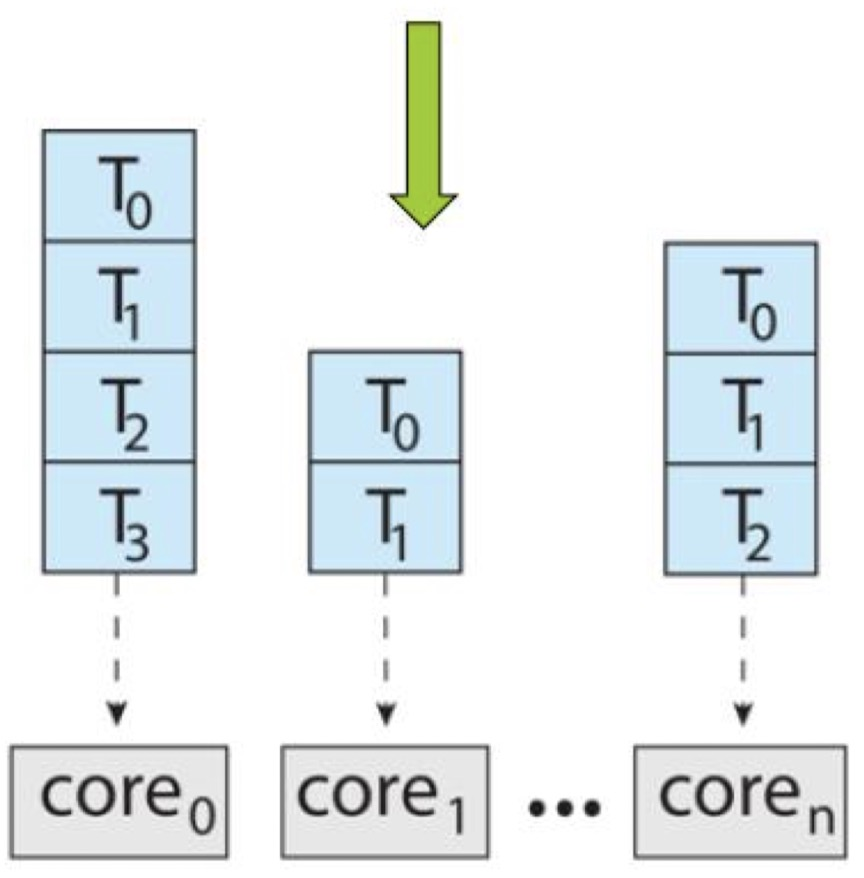
\includegraphics[width=0.3\linewidth]{assets/one-queue-one-core.jpg}
          \end{figure}

          \begin{note}
              In questo caso risulta essere importante ripartire uniformemente il carico tra i vari processori.

              Un controllo delle lunghezze delle code avviene sia periodicamente sia quando un determinato processore diventa inattivo.
          \end{note}

    \item Una singola coda per tutti i processori, questo risolve il problema del bilanciamento, ma genera delle race condition nell'accesso alla struttura dati.
          \begin{figure}[H]
              \centering
              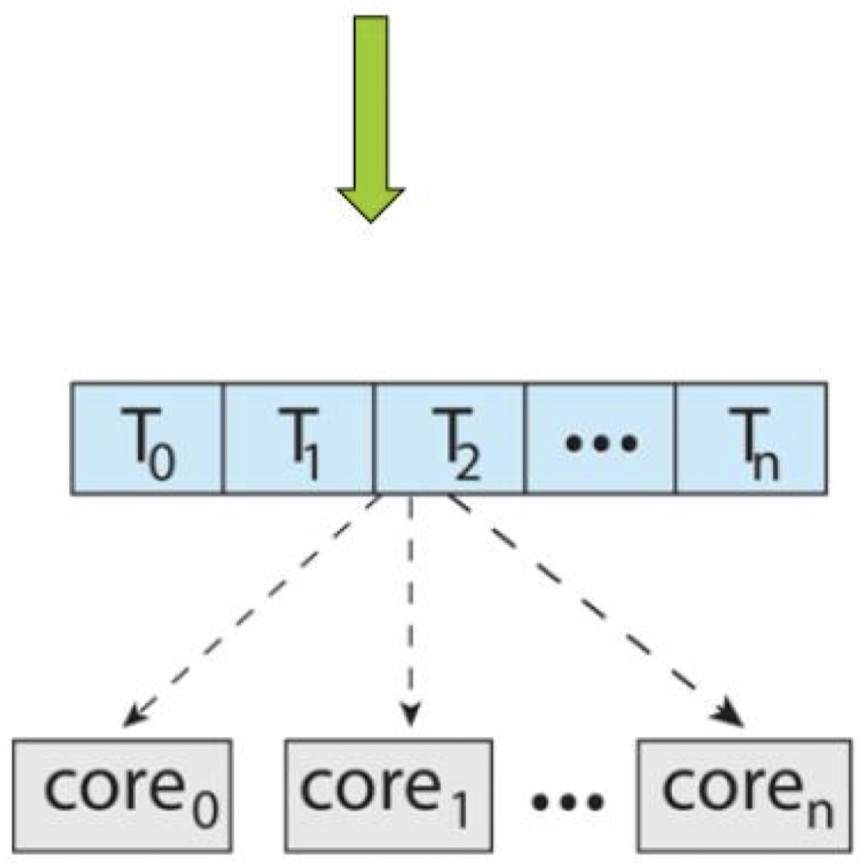
\includegraphics[width=0.3\linewidth]{assets/one-queue-many-core.jpg}
          \end{figure}
\end{itemize}

Esistono alcuni processi che hanno una predilezione per essere eseguiti sempre nello stesso core, questo permette loro di sfruttare al meglio la cache, ma non è sempre supportata dal sistema operativo.

\subsubsection*{Bilanciamento del Carico}
È il procedimento che permette di ripartire uniformemente il carico di lavoro tra più processori, può essere implementata in due modi:
\begin{sitemize}
    \item \textbf{Migrazione Guidata:} Un processo dedica controlla periodicamente il carico dei processori per correggere anticipamente gli equilibri
    \item \textbf{Migrazione Spontanea:} Un processore inattivo sottrae ad uno sovraccaricato un processo tra quelli in attesa.
\end{sitemize}

\subsection{Implementazioni}
\subsubsection{Linux}
Prima della versione 2.5 il kernel Linux implementava delle code multiple gestite perlopiù in Round Robin. La priorità viene calcolata periodicamente in base a quante risorse un processo ha consumato dall'ultimo controllo, minori sono le risorse utilizzate, maggiore sarà la priorità.

\spacer
Dalla versione 2.6.23 il kernel Linux implementa due code, \textit{default} e \textit{real-time}, con uno scheduler \textit{CFS (Completely Fair Scheduler)} che assegna ad ogni task una percentuale del tempo di CPU.

A ciascuna task viene associata una priorità (-20 a +19)

\spacer
Lo scheduler associa ad ogni task il suo tempo di esecuzione virtuale, una quantità che tiene conto sia del tempo di esecuzione che della priorità della task. Quindi una task a bassa priorità avrà un \texttt{vruntime} maggiore di una a priorità più alta, anche se sono state entrambe eseguite per lo stesso tempo.
Lo scheduler poi esegue la task con il valore \texttt{vruntime} più basso.

\spacer
Lo scheduler Linux è ottimizzato anche per sistemi NUMA, implementando delle strategie per ridurre al minimo il numero di migrazione dei processi da un processore all'altro.

\spacer
Le CPU Alder Lake causano non pochi problemi allo scheduler Linux < 5.16, infatti esso non si aspetta di vedere processori con livelli di prestazione diversi, ottimizzati per diverse situazioni.

\subsubsection{Windows 10}
Implementa livelli di priorità da 0 a 31, ogniuno con la sua coda. Lo scheduler poi seleziona l'ultimo processo dalla coda a priorità più alta non vuota.

\spacer
I thread che hanno una priorità compresa tra 0 e 15 vengono gestiti dinamicamente, quando uno di essi viene portato in foreground, oppure riceve un input dall'utente, la sua priorità viene aumentata.

Inoltre la priorità dinamica viene diminuita di un livello ogni volta che il processo accede alle risorse della CPU, fino a tornare alla priorità base.

\subsubsection{Windows 11}
Windows 11 è stato scritto pensando alle nuove CPU intel, le quali hanno dei core ad alte prestazioni e degli altri ad alta efficienza.

Lo scheduler del sistema interagisce attivamente con un microcontrollore integrato nella CPU, chiamato \textit{Thread Director}.

Esso comunica al sistema operativo dei consigli sulla gestione dei processi processi prendendo in considerazione la situazione attuale del processore.

\spacer
Un'altra funzionalità introdotta da Windows 11 è il GPU accelerated scheduler, esso permette alla GPU di autogestire alcune task e la sua VRAM, alleggerendo il carico sulla CPU.

\subsubsection{Sistemi Real Time}
I sistemi operativi real time si dividono in:
\begin{sitemize}
    \item \textbf{Hard Real Time:} Richiedono il completamento di alcuni processi critici entro limiti specifici.
    \item \textbf{Soft Real Time:} Richiedono solo che ad alcuni processi venga fornita una priorità maggiore.
\end{sitemize}
